\documentclass{article}
\usepackage{fullpage}
\usepackage{enumitem} 	% For custom labelling of enumerate
\usepackage{amsthm} 	% For creation of custom theorem-like environments 
\usepackage{amssymb}	% For usage of mathbb for the reals symbol
\usepackage{amsmath}	% For usage of align* environment
\usepackage{siunitx}	% For usage of \SI and \num for scientific notation
\usepackage{graphicx}	% For inclusion of images
\usepackage{float}		% For usage of [H] tag to force position
\usepackage{subcaption}


% Forces enumerate to follow these indentations
% Also possible to use \setlength above and then refer to \parskip or \parindent below
\setenumerate{parsep = 3ex, listparindent = 2em}

\title{Team MagicMarijuanaForest: Movie Visualizations}
\author{Zhewei Chen, Milad Taghavi, and Yan Qi Huan}


\begin{document}
	\maketitle

	\section{Basic Visualizations}
		\begin{figure}[H]
			\centering
			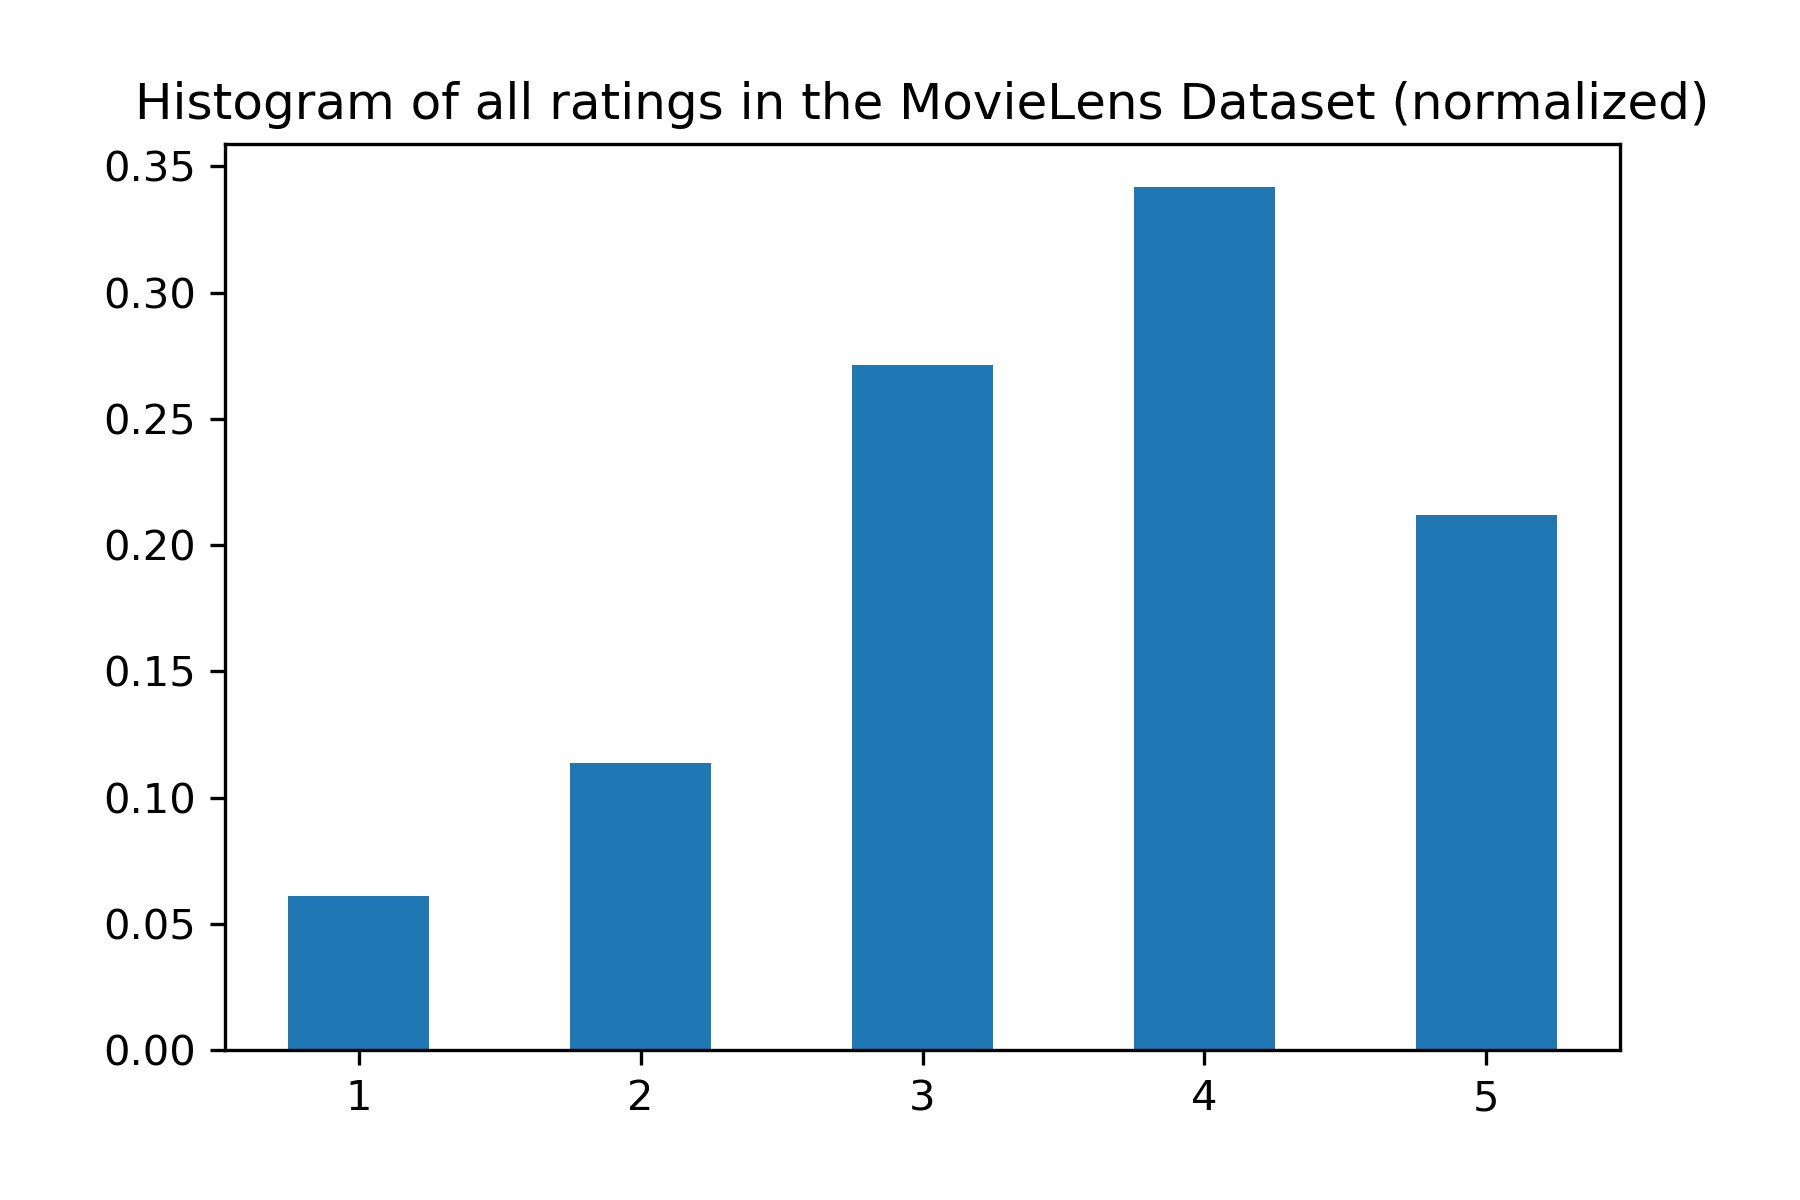
\includegraphics[width=0.5\textwidth]{Fig4-1.png}
			\caption{4.1: All ratings in the MovieLens Dateset. We plot the number of ratings with a particular score as a normalized histogram.}
		\end{figure}
	
	\begin{figure}[H]
		\centering
		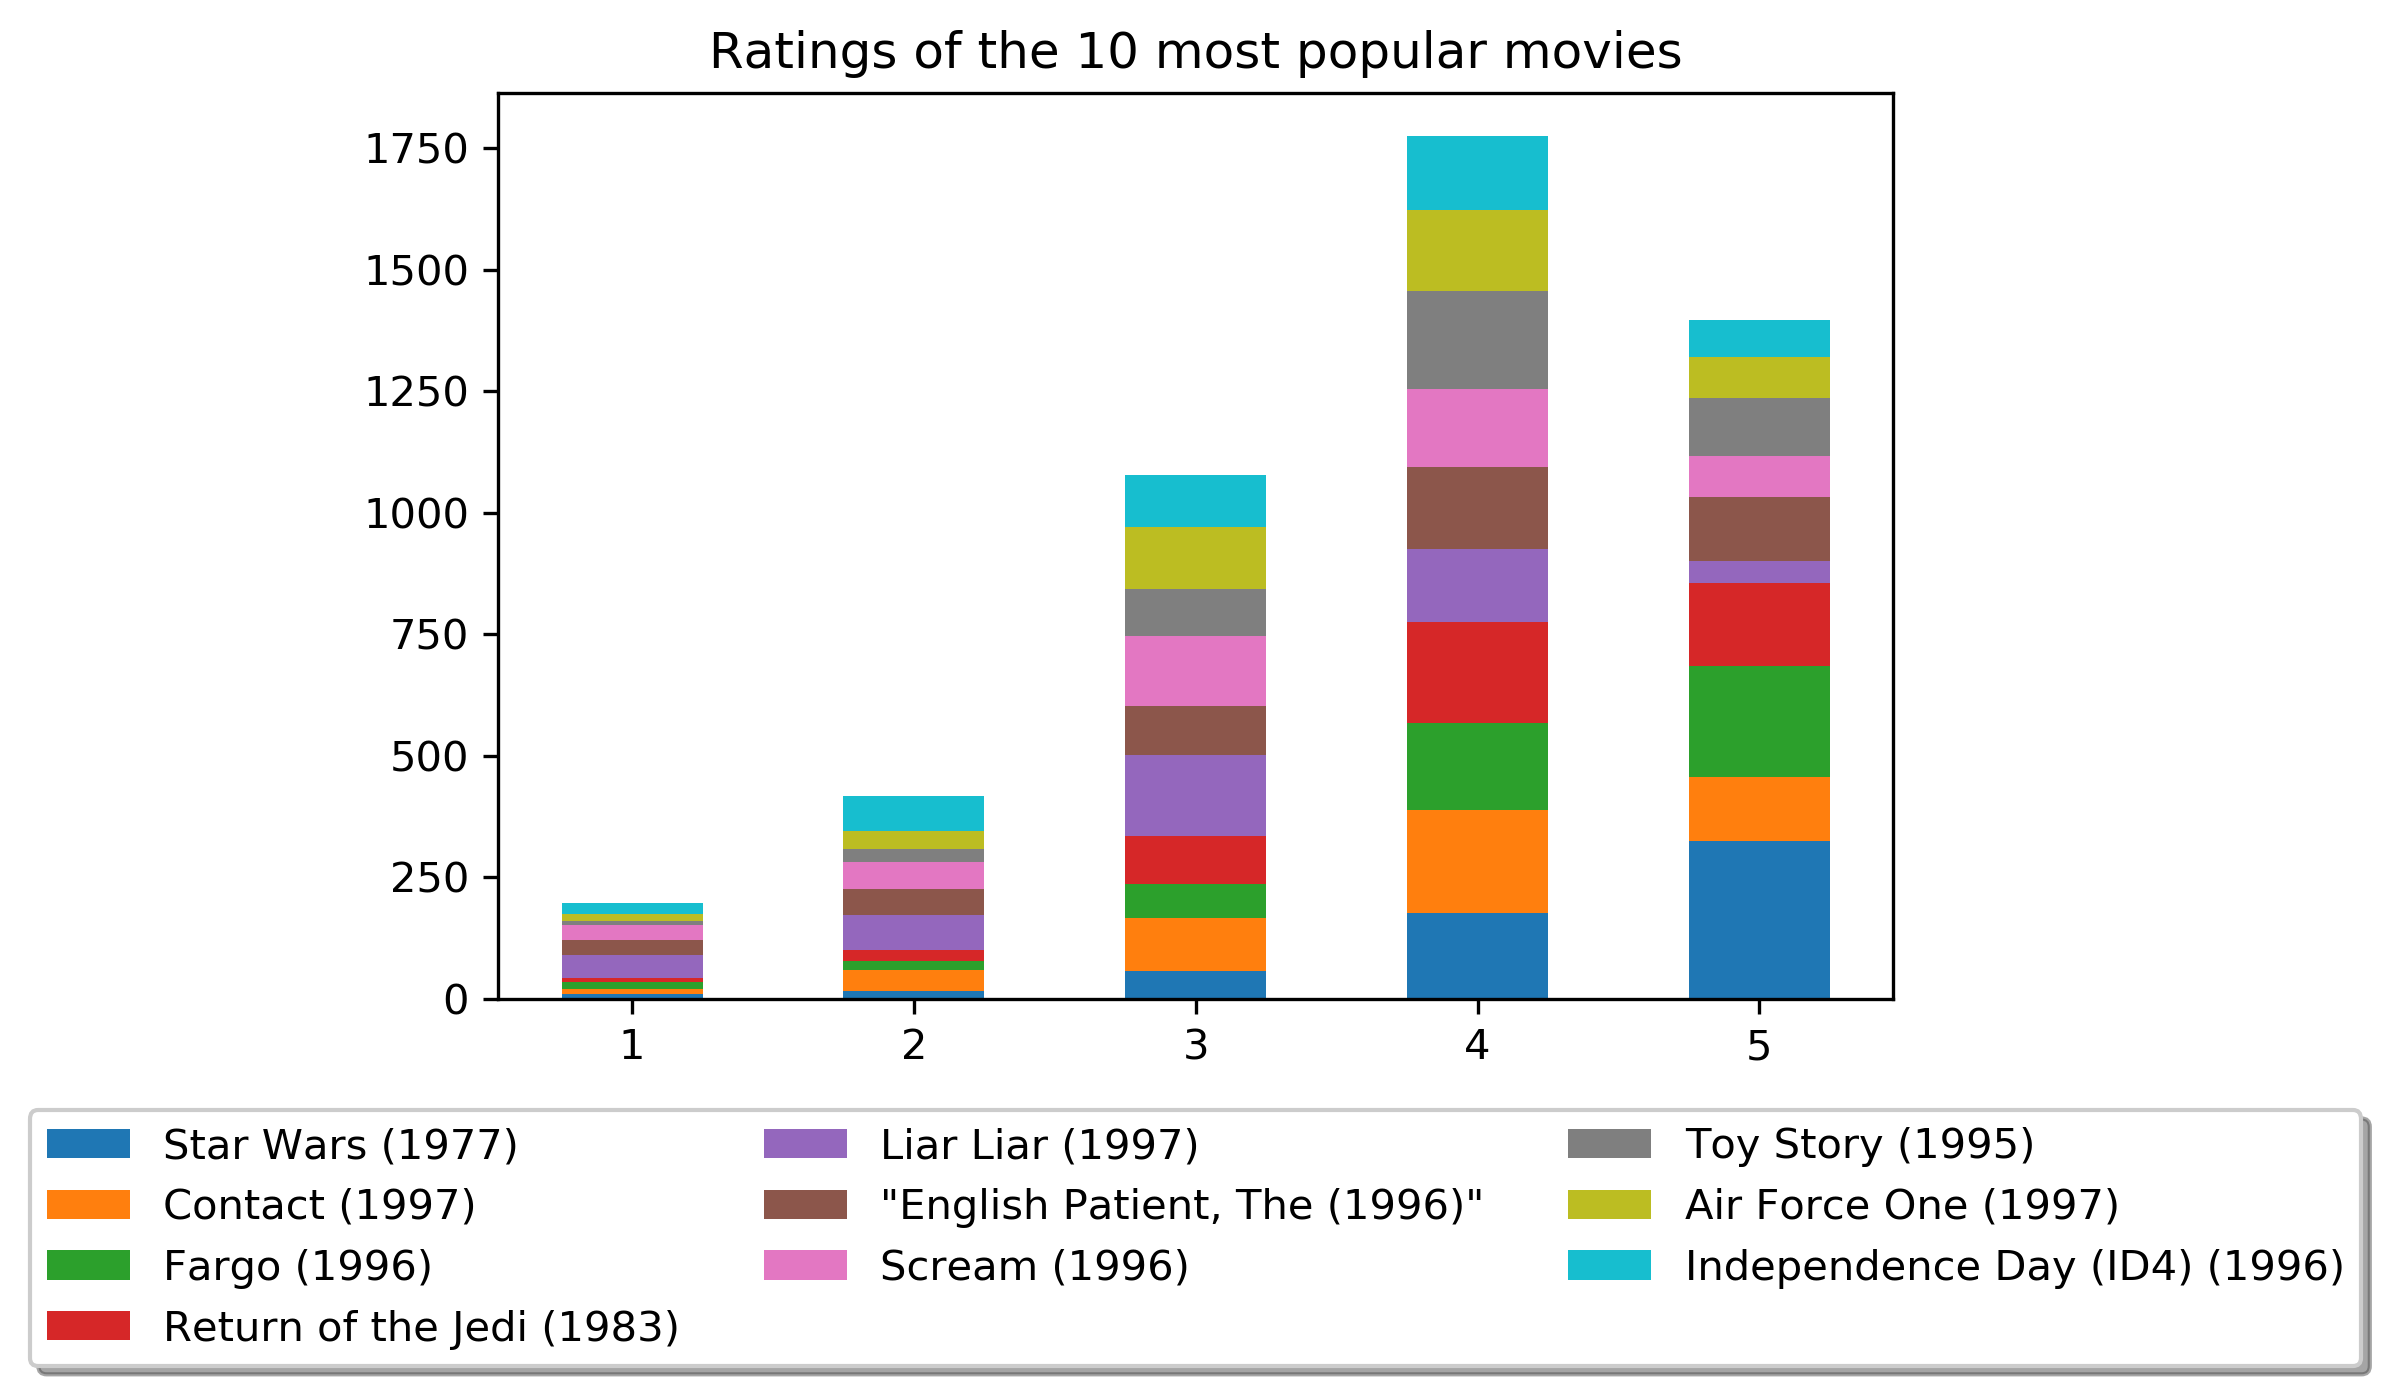
\includegraphics[width=0.7\textwidth]{Fig4-2.png}
		\caption{4.2: All ratings of the top 10 most popular movies. We plot the normalized review counts for each of the 10 movies against the score of each review.}
	\end{figure}

	\begin{figure}[H]
	\centering
	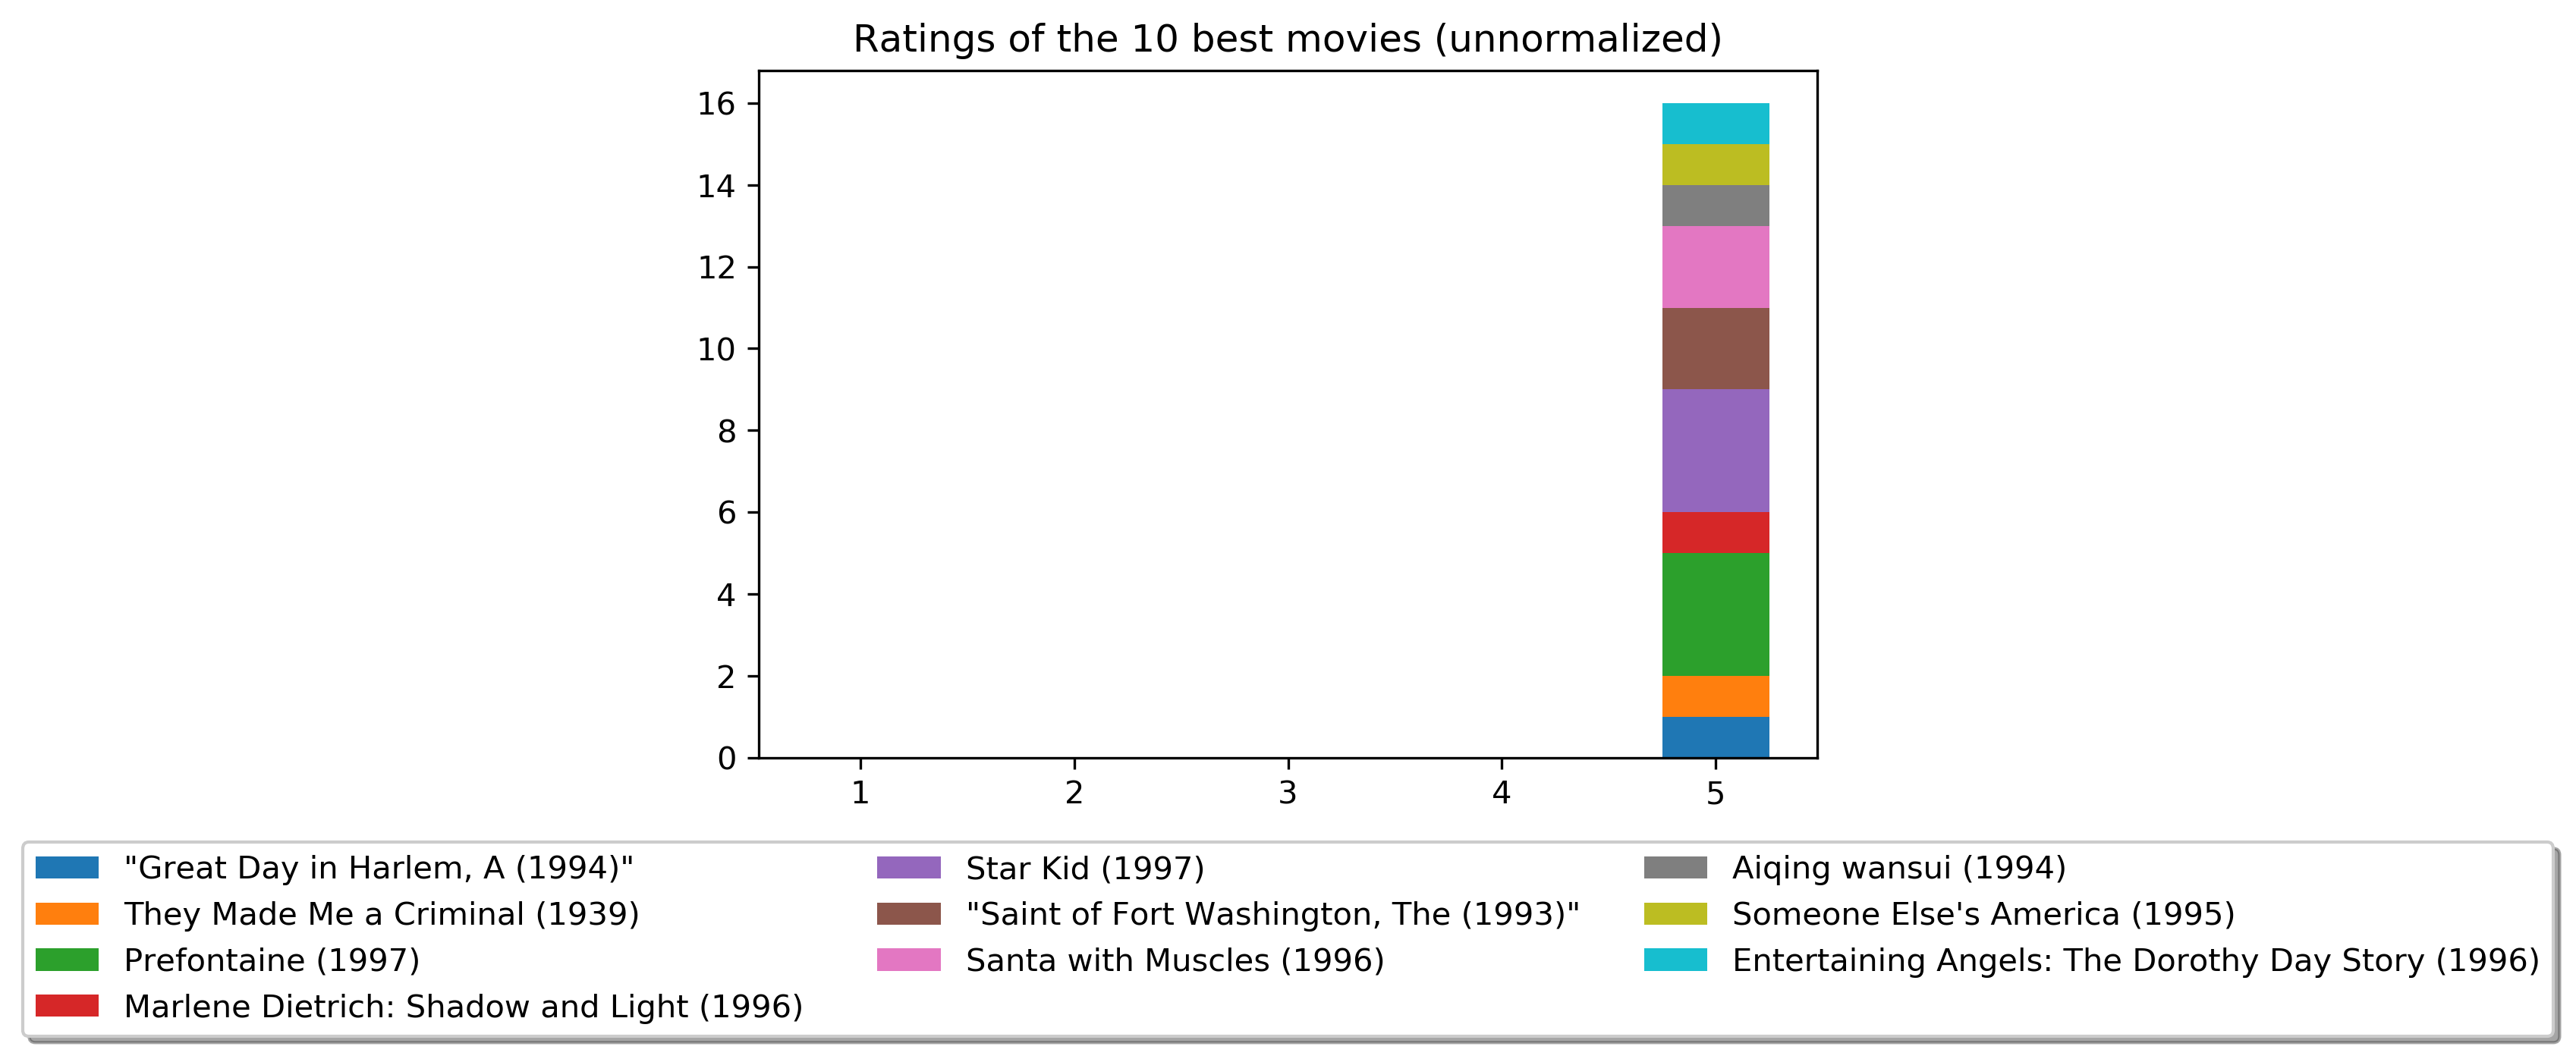
\includegraphics[width=0.8\textwidth]{Fig4-3.png}
	\caption{4.3: All ratings of the movies with the top average scores. We use an unnormalized histogram in this case since each movie only has reviews that give it a score of 5. Note that all these movies have less than 5 reviews.}
	\end{figure}

\begin{figure}[H]
	\centering
	\begin{subfigure}[t]{0.3\textwidth}
		\centering
		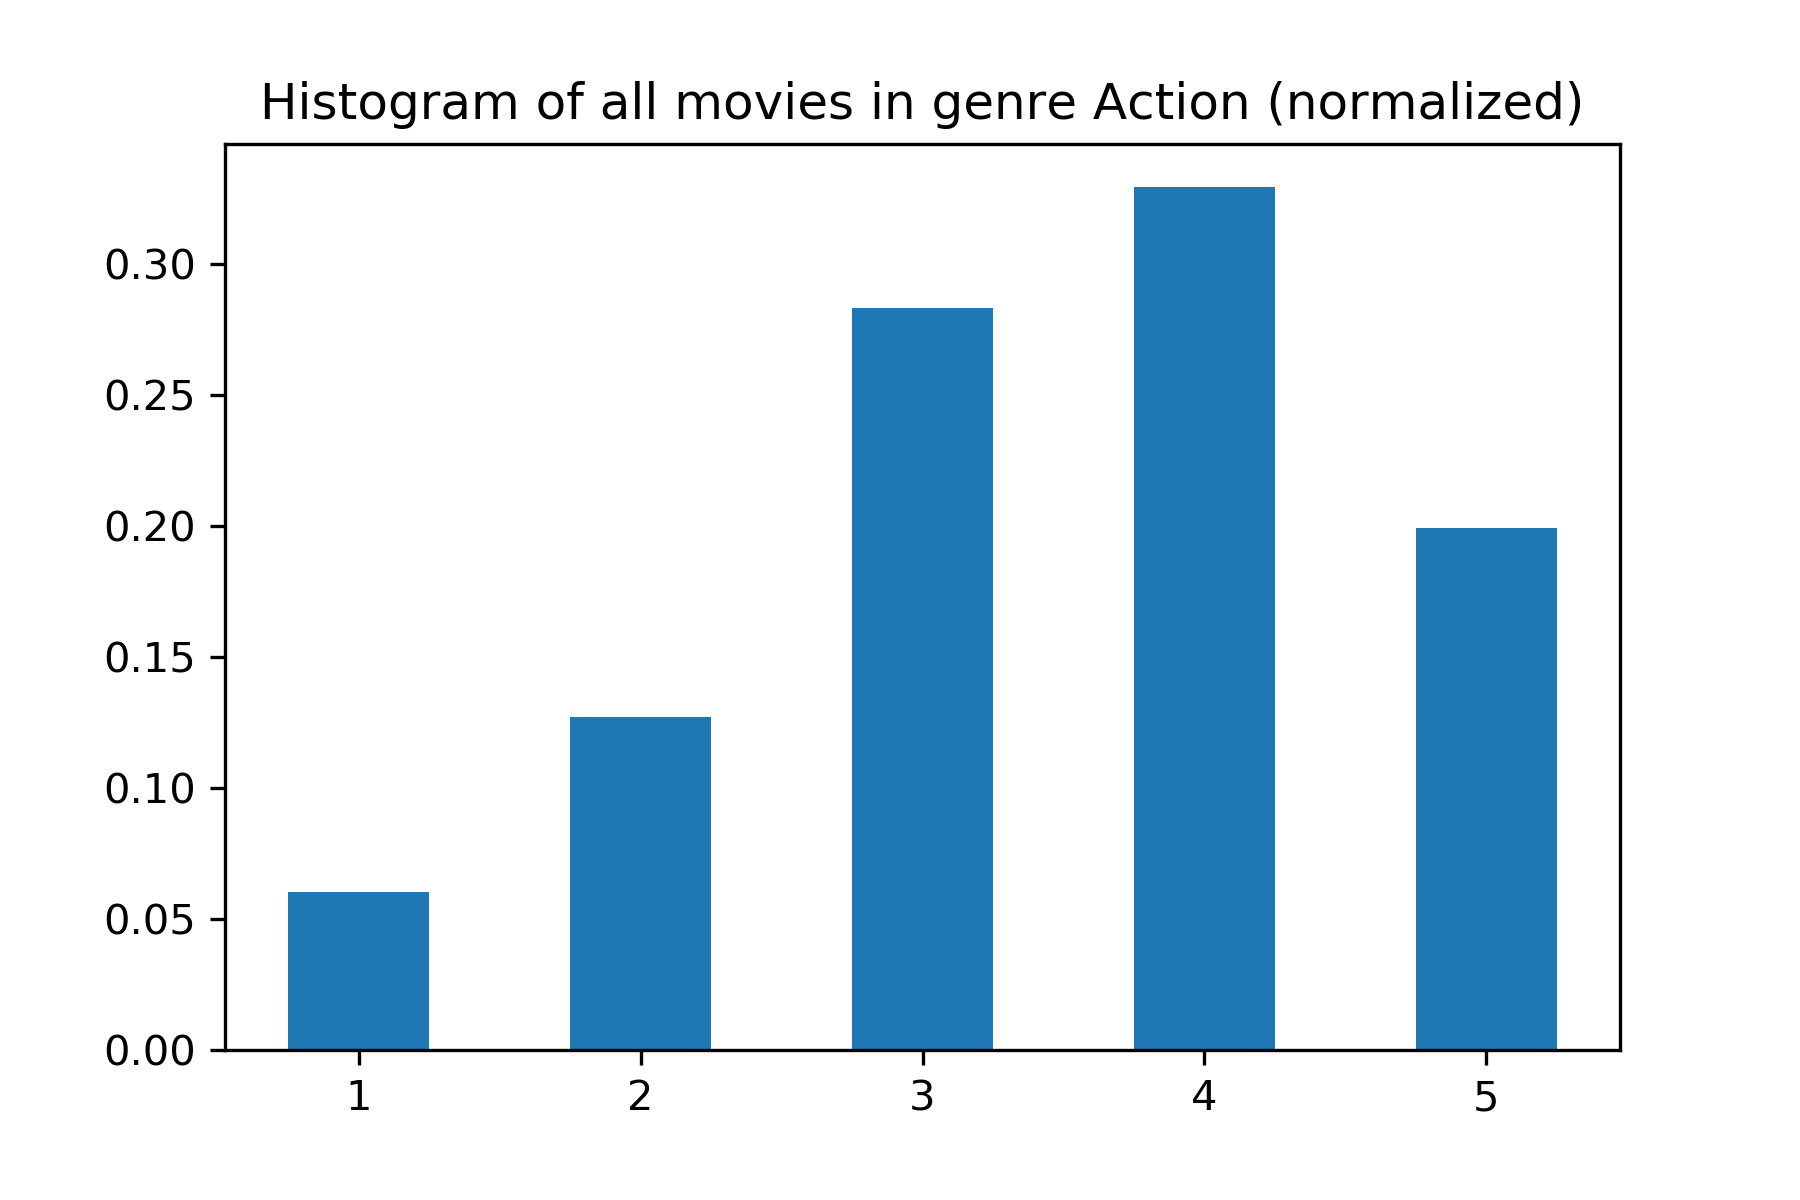
\includegraphics[width=\textwidth]{Fig4-4-1}
		\caption{Action genre}
	\end{subfigure}%
	~ 
	\begin{subfigure}[t]{0.3\textwidth}
		\centering
		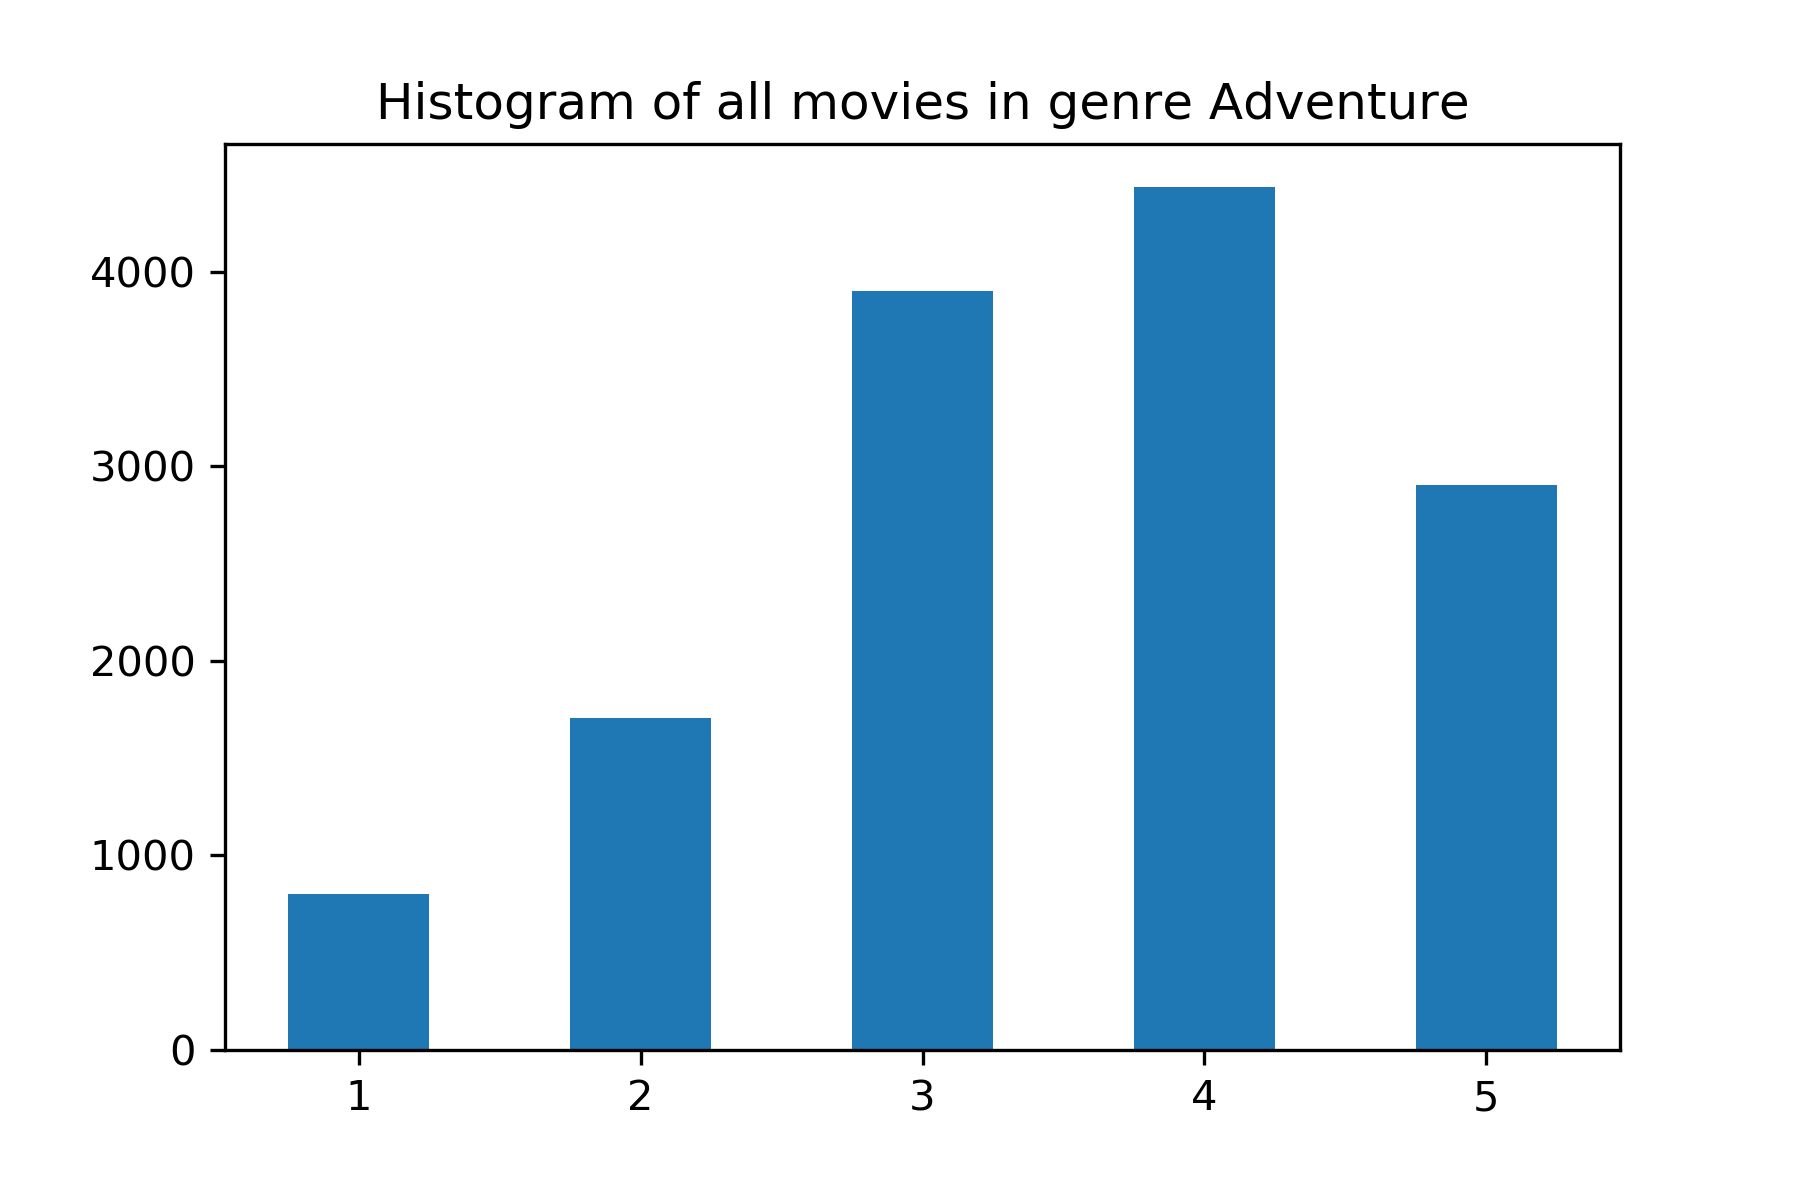
\includegraphics[width=\textwidth]{Fig4-4-2}
		\caption{Adventure genre}
	\end{subfigure}
	~
	\begin{subfigure}[t]{0.3\textwidth}
		\centering
		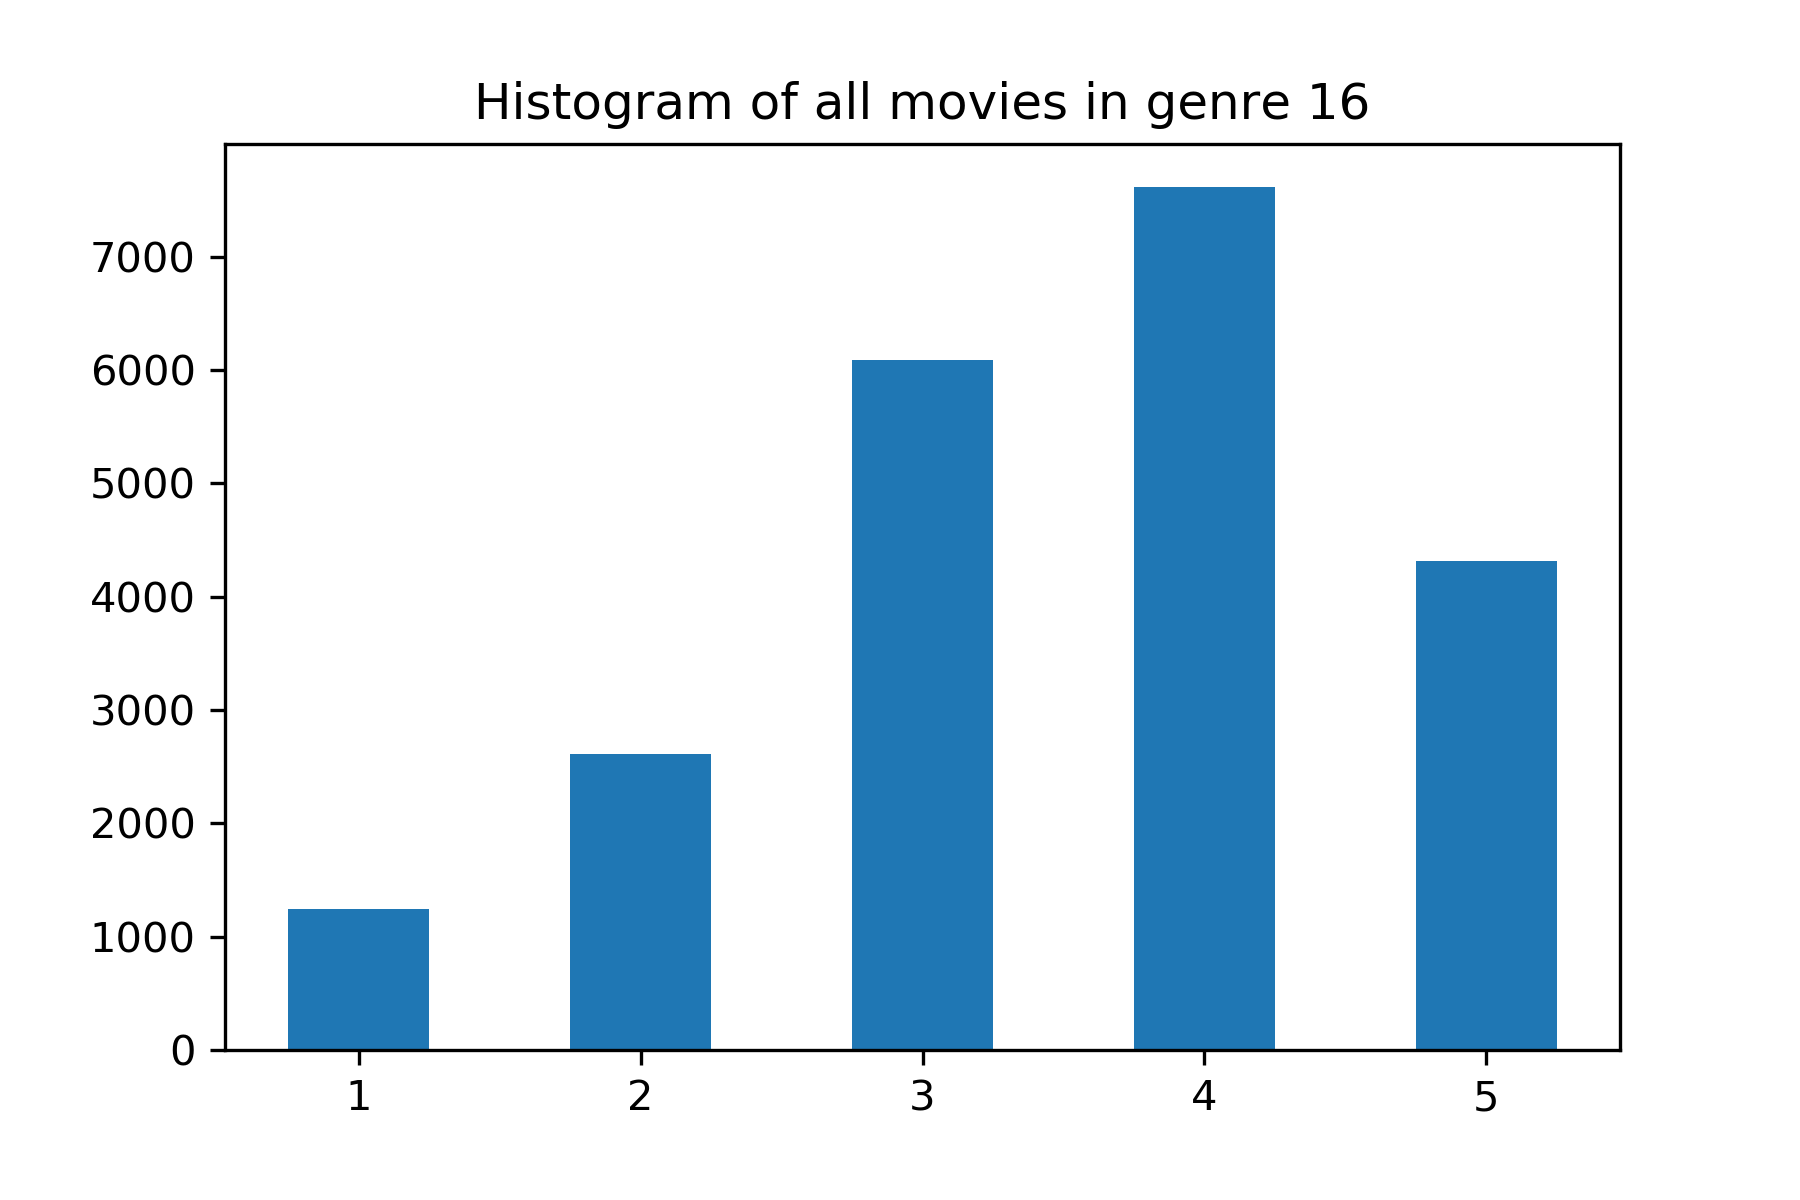
\includegraphics[width=\textwidth]{Fig4-4-3}
		\caption{War genre}
	\end{subfigure}
	\caption{4.4: Normalized histogram of scores for movies from the genres Action, Adventure and War.}
\end{figure}

	\begin{figure}[H]
	\centering
	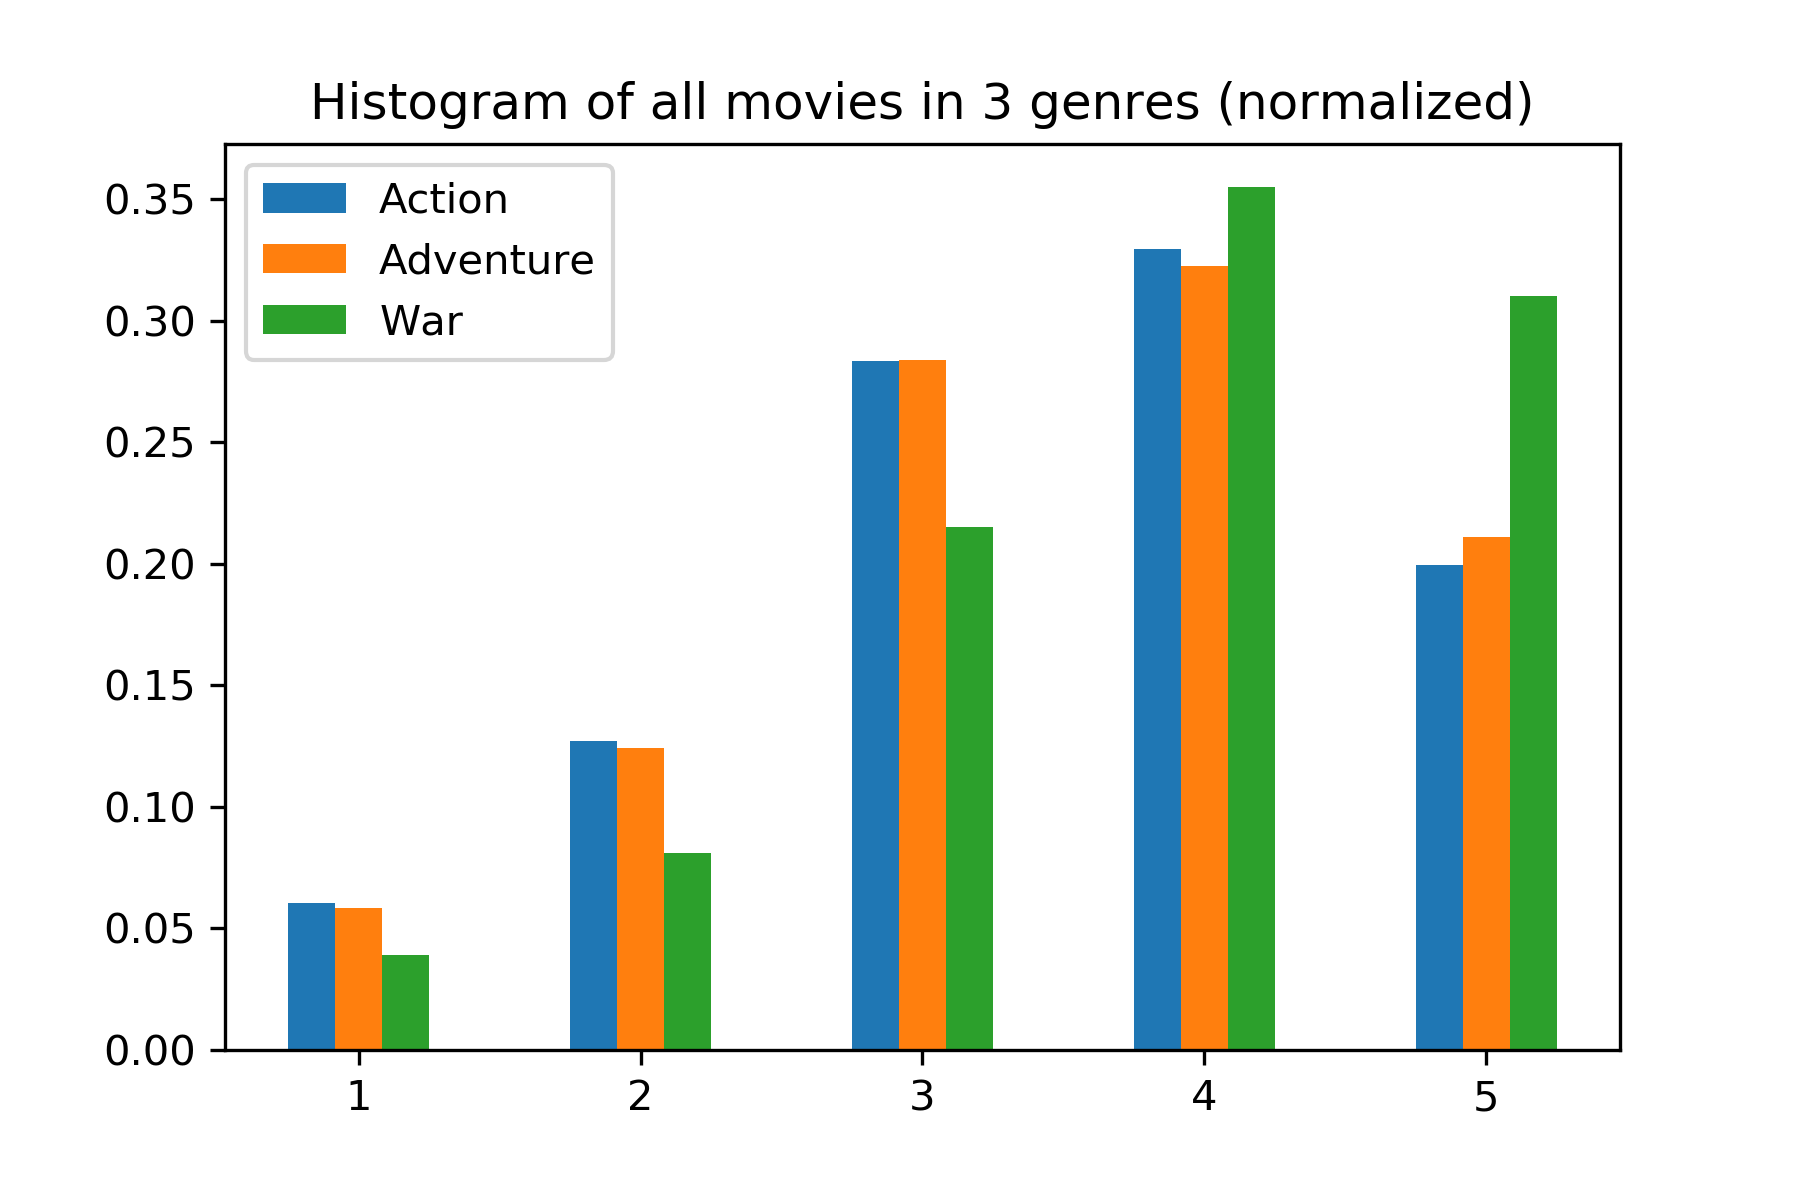
\includegraphics[width=0.5\textwidth]{Fig4-4-4.png}
	\caption{4.4: In order to compare the 3 genres, we also plotted them side by side in a combined histogram.}
\end{figure}

\section{Matrix Factorization Visualizations}
\begin{figure}[H]
	\centering
	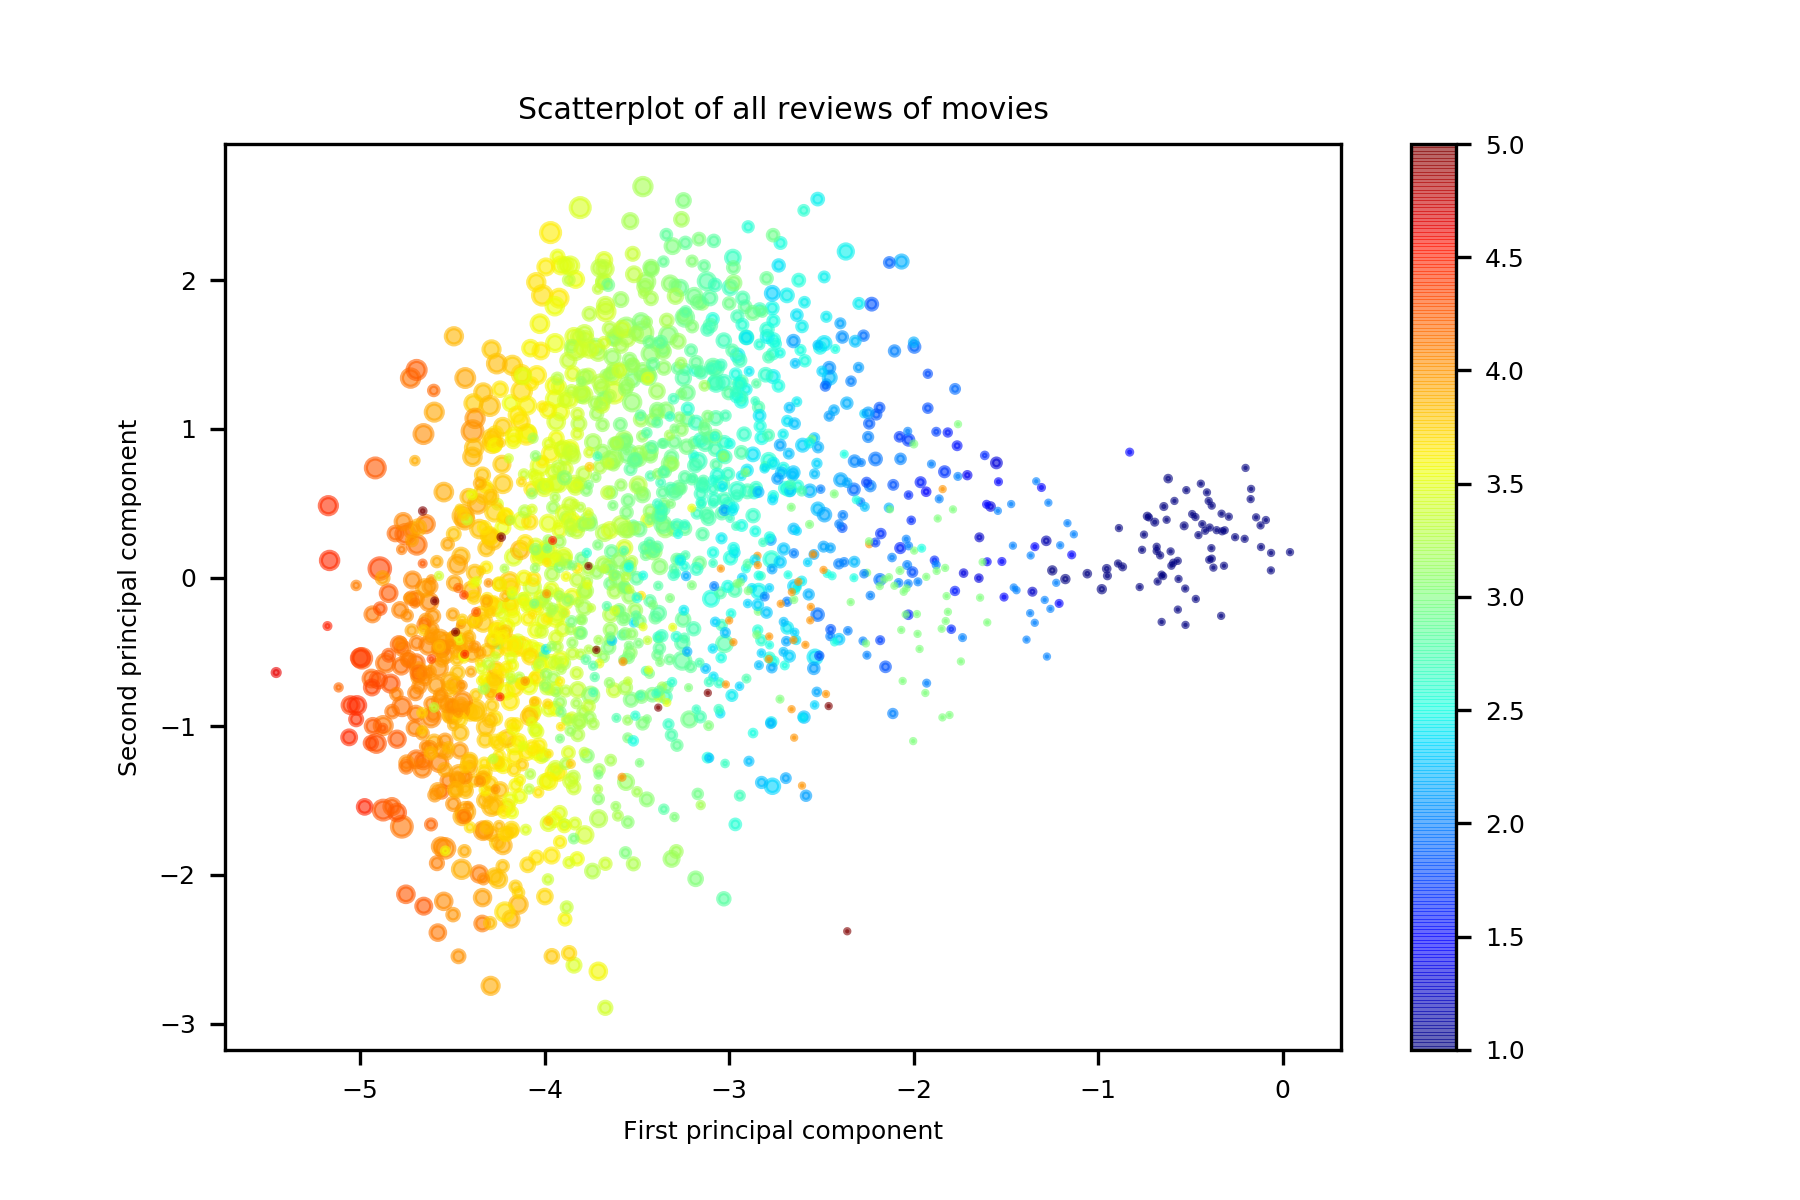
\includegraphics[width=0.5\textwidth]{ScoresRaw.png}
	\caption{This scatter plot of each movie vector projected onto the first two principal components of the latent movie matrix. Ratings (color bar) are strongly determined by the first principal component. The size of the data point corresponds to the number of ratings given to that movie.}
\end{figure}


\begin{figure}[H]
	\centering
	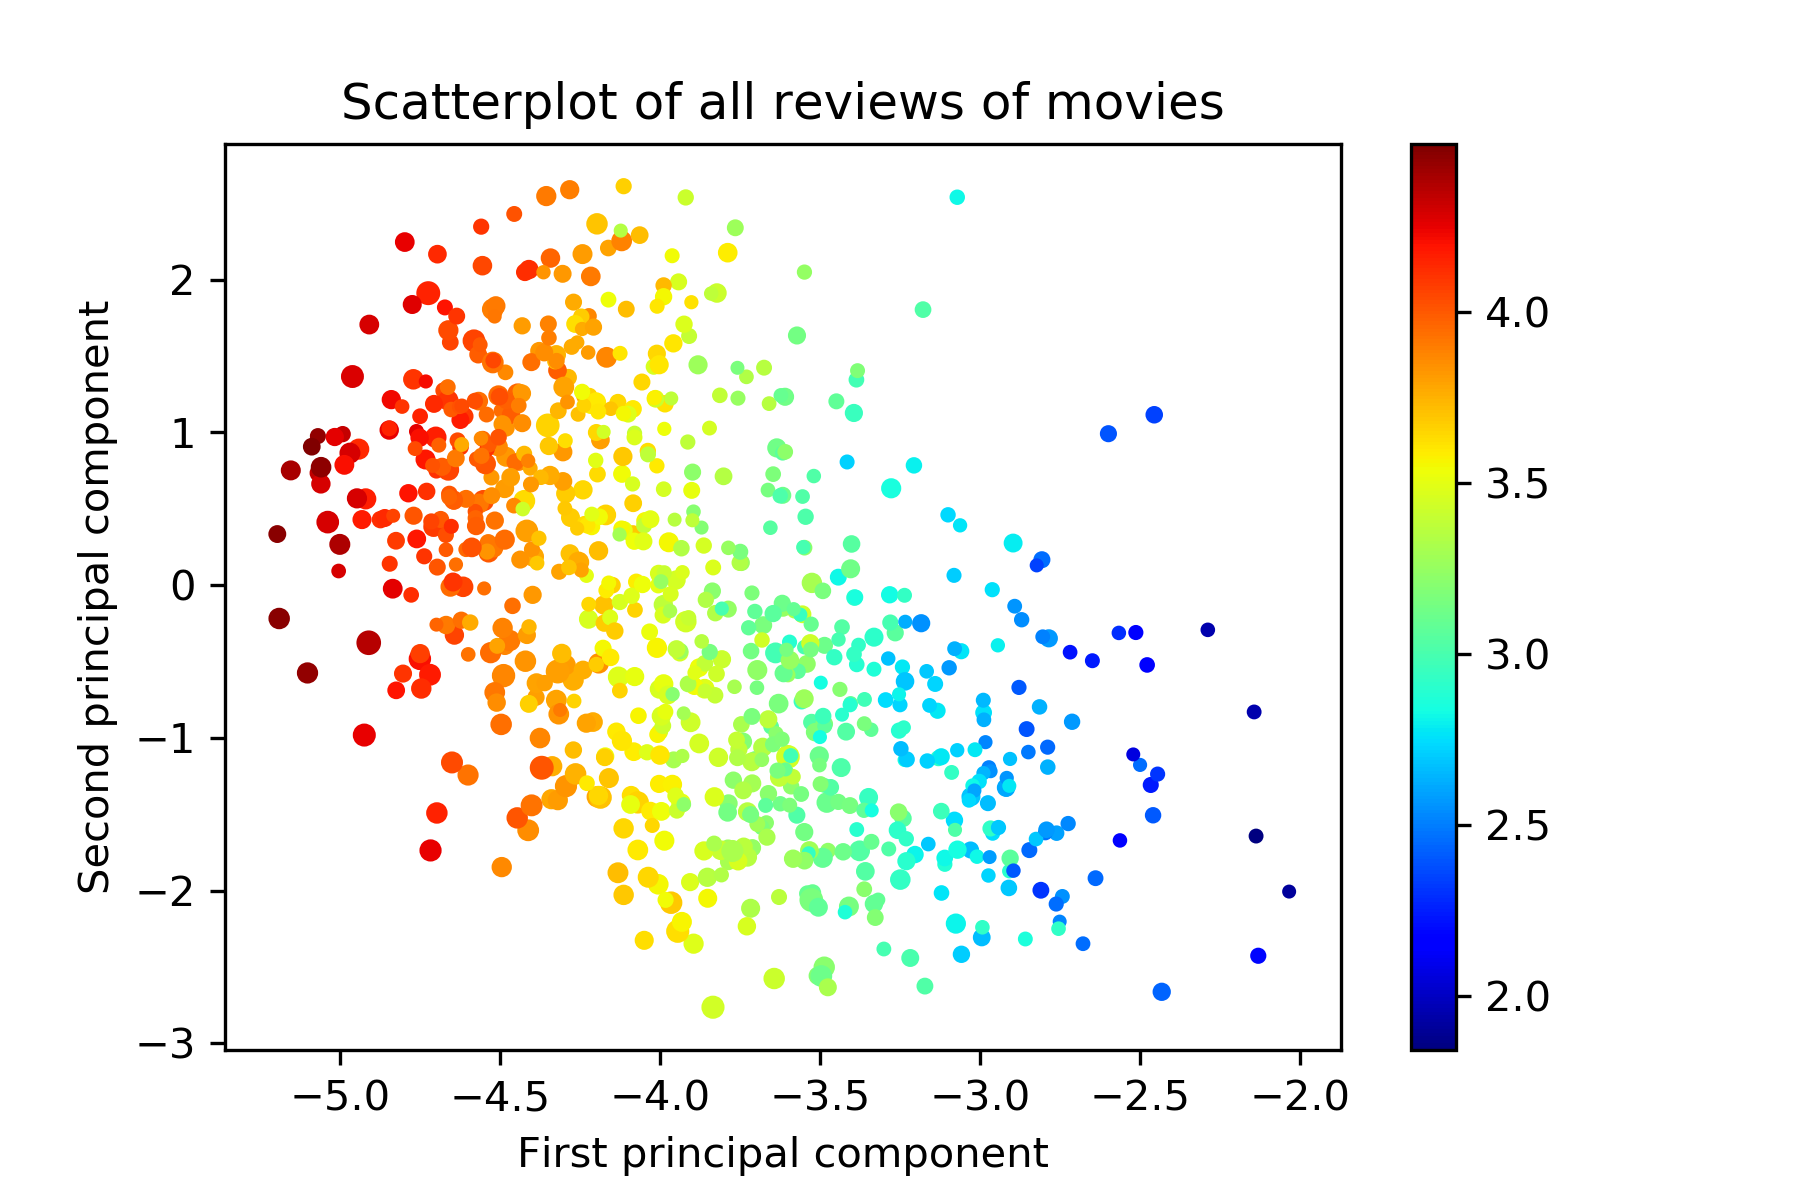
\includegraphics[width=0.5\textwidth]{Scores30Raw.png}
	\caption{In this figure movies with less than 30 reviews are filtered out from the previous plot. As a result of this filtering, the island of movie vectors disappears. The isolated red dots (highly rated movies, but few reviews) also disappear.}
\end{figure}


\begin{figure}[H]
	\centering
	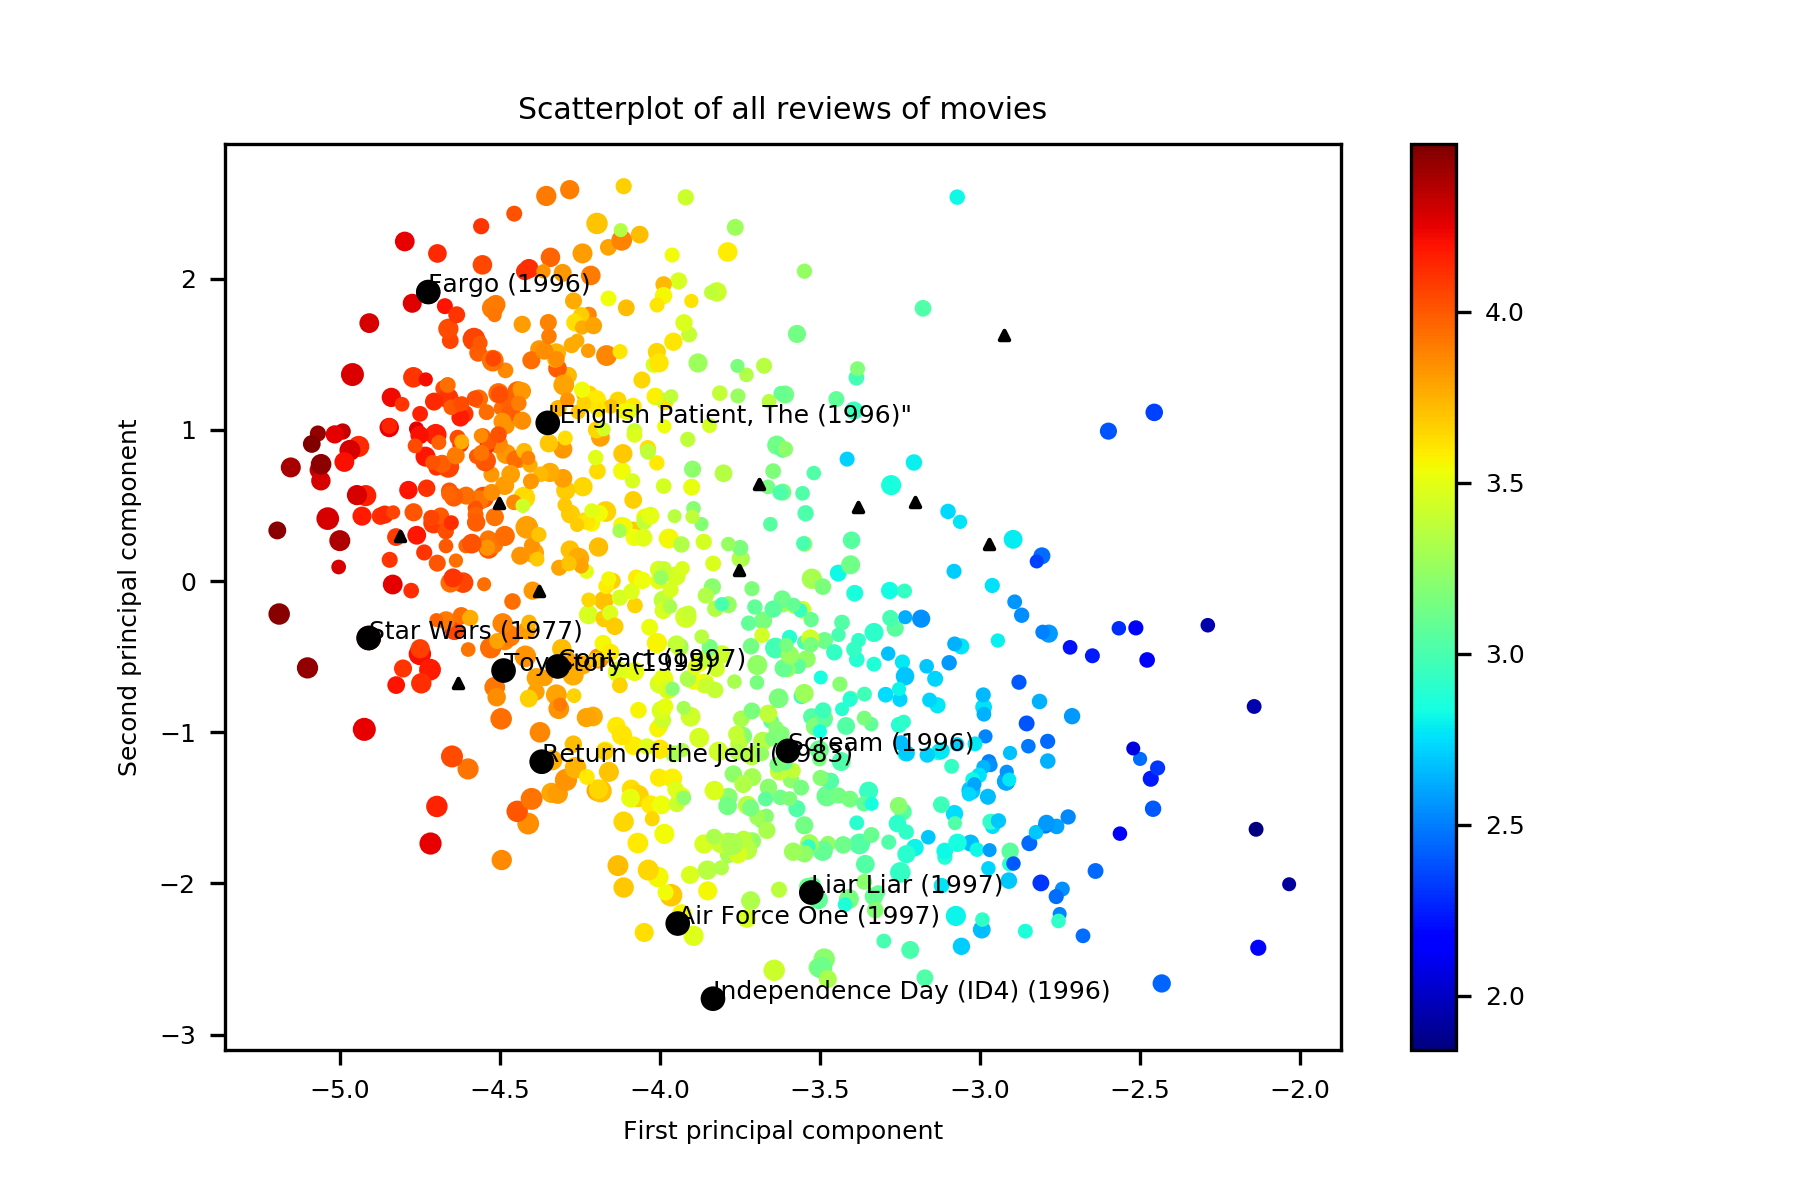
\includegraphics[width=0.5\textwidth]{Scores30Labelled.png}
	\caption{Here the top ten most rated movies marked in black circles. The top ten most highly rated movies are in black triangles. The size of the markers correspond to the number of ratings. Here we also excluded movies which have less than 30 reviews to filter out potentially noisy outlier movie ratings.
	}
\end{figure}

\begin{figure}[H]
	\centering
	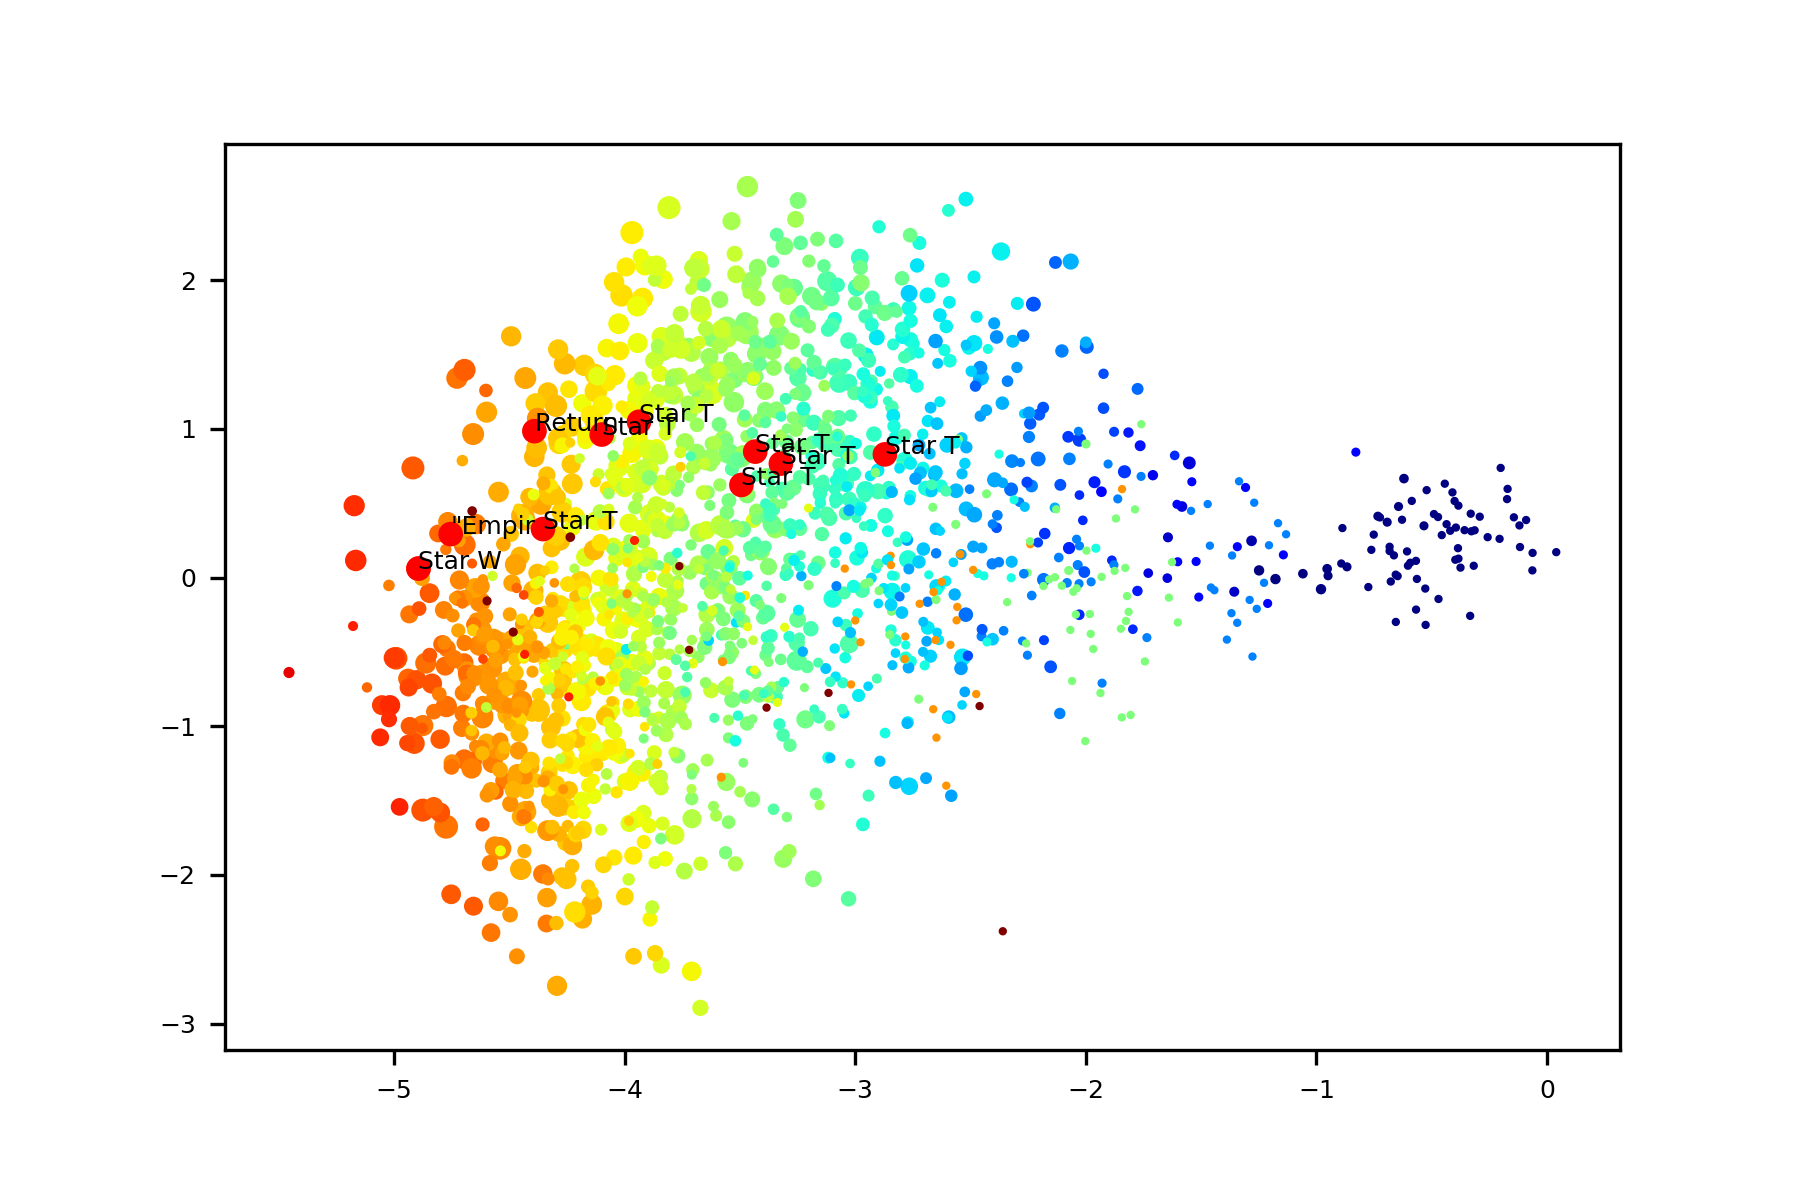
\includegraphics[width=0.7\textwidth]{Star.png}
	\caption{10 movies of our choice - 3 were from Star Wars and the remaining 7 were from Star Trek (Names are shortened due to space constraints). We see that these generally tend to congregate in the bottom left quadrant of the plot, indicating the expected similarity between these movies. There is also a weak separation between the Star Wars movies and the Star Trek movies.
	}
\end{figure}

\begin{figure}[H]
	\centering
	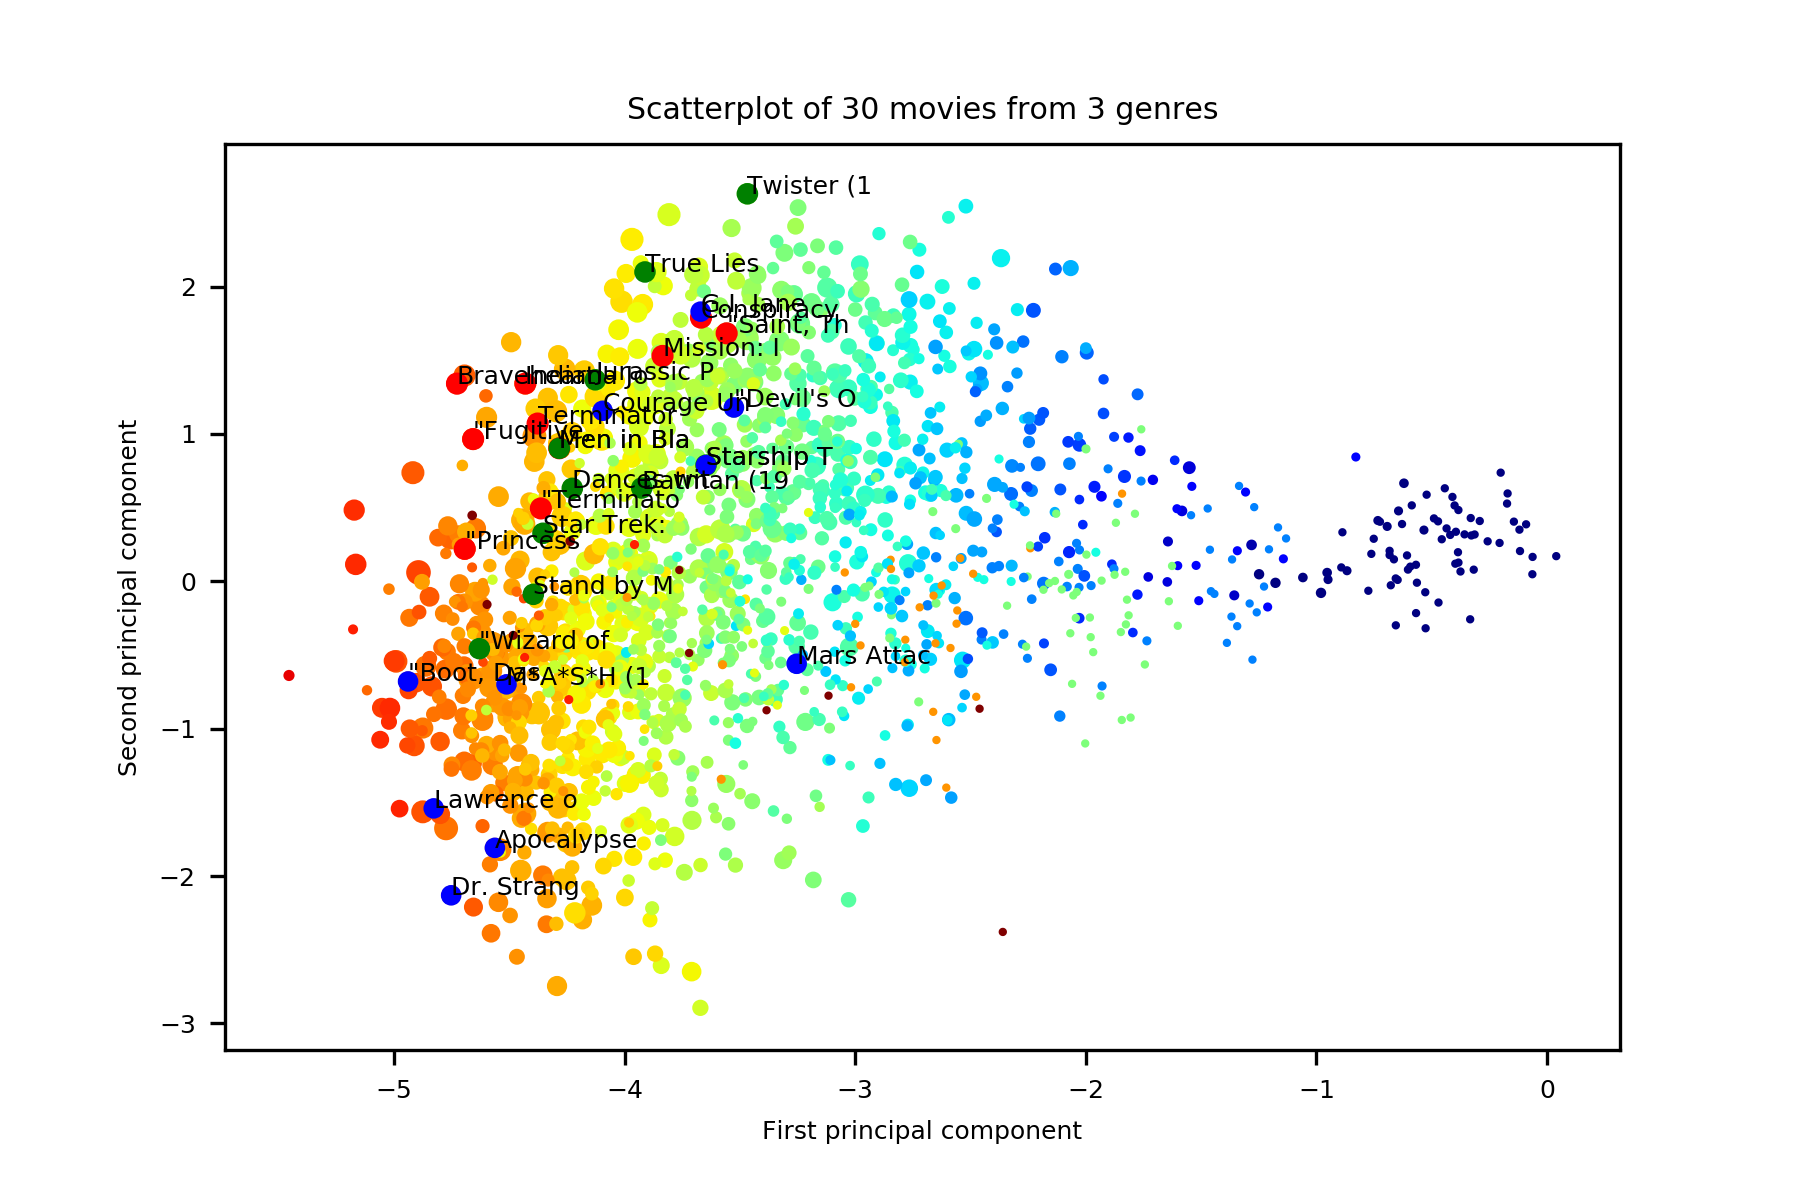
\includegraphics[width=0.7\textwidth]{3Genres.png}
	\caption{Scatter plot of 10 movies from 3 genres: Action (Red), Adventure (Green), and War (Blue). Movie names are shortened due to space constraints. The movies chosen were the 10-20th most rated for each genre (we omitted the top 10 to avoid using the same points as Figure 8). 
	}
\end{figure}


\section{Other Interesting Visualizations}


\begin{figure}[H]
	\centering
	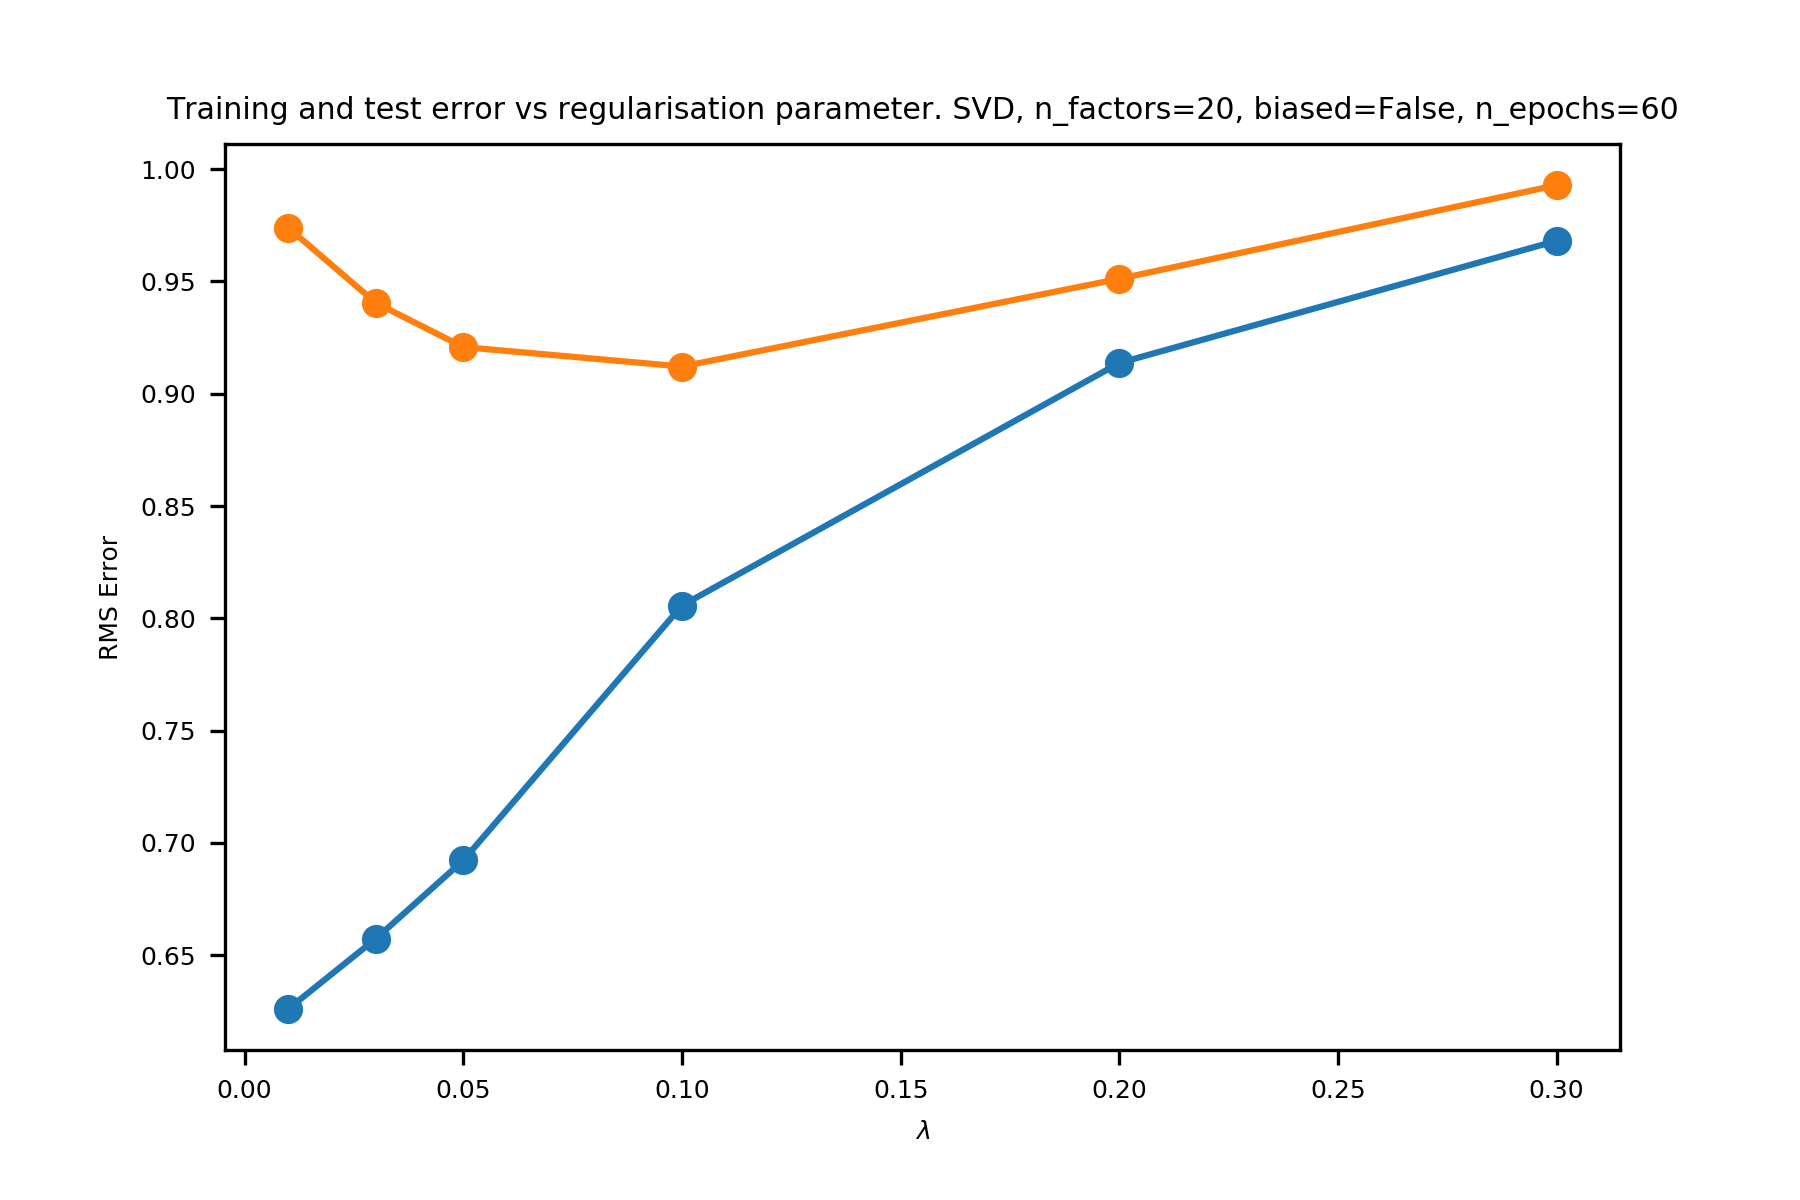
\includegraphics[width=0.5\textwidth]{SVDNoBias_RegErr.png}
	\caption{Learning curve of matrix factorization as a function of regularization parameter $\lambda$. The optimal parameter was chosen as 0.1.
	}
\end{figure}


\begin{figure}[H]
	\centering
	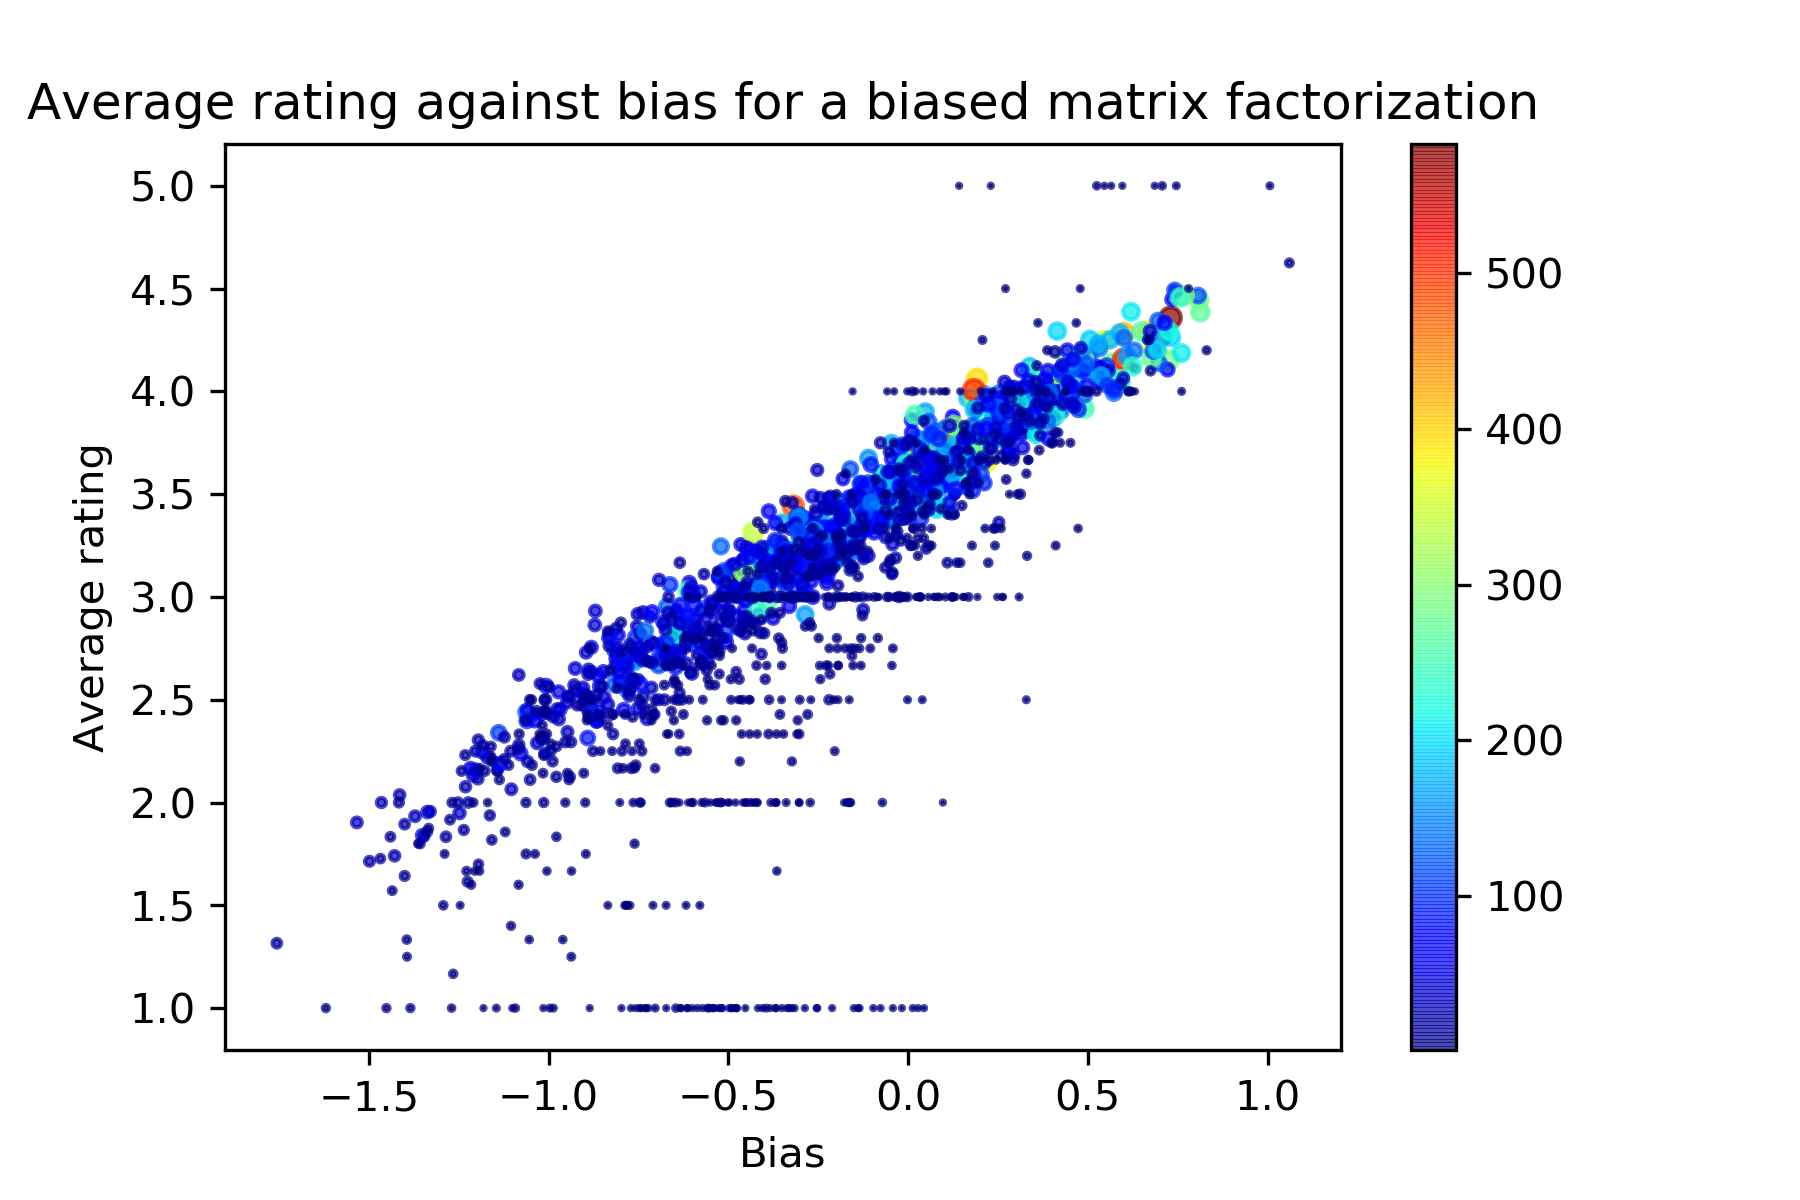
\includegraphics[width=0.7\textwidth]{RatingVsBias.png}
	\caption{A variant of the model with biases in the weights was also tried. This plot shows a strong monotonic dependence of the average rating of a movie with the bias weight.
	}
\end{figure}

\begin{figure}[H]
	\centering
	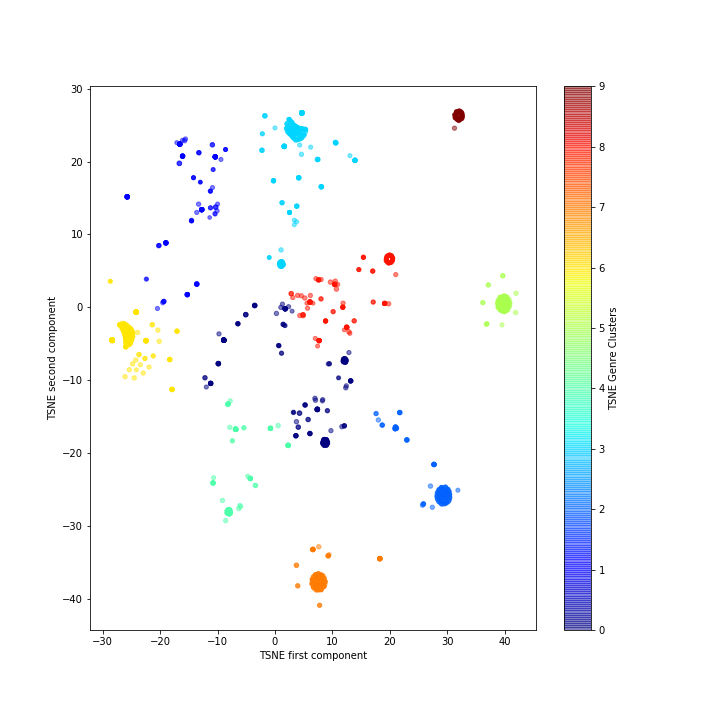
\includegraphics[width=0.7\textwidth]{TSNEcluster.png}
	\caption{The genres that each movie belonged to were first processed using t-SNE (t-distributed Stochastic Neighbor Embedding) to compress the high-dimensional vectors into a 2-dimensional representation. Clustering (with a choice of $k=10$ clusters) was then done on this representation.
	}
\end{figure}

\begin{figure}[H]
	\centering
	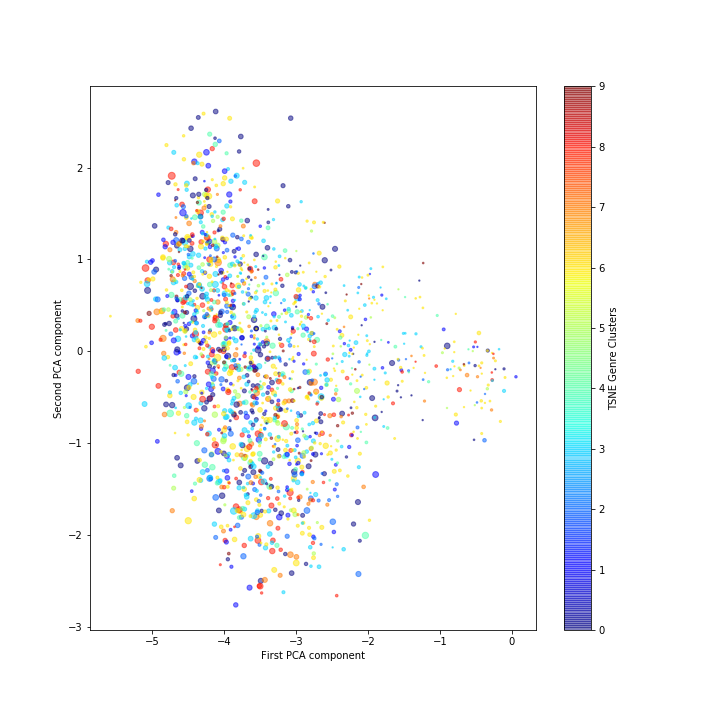
\includegraphics[width=0.7\textwidth]{TSNE_PCA_cluster.png}
	\caption{The clustering from the previous figure was then overlaid onto first 2 PCA components of the V matrix of the movie vectors (colours represent the genre cluster that the movie belongs to, size represents the number of ratings). We observe no clear trend between genre cluster and the PCA components. We hypothesize that this is due to the fact that there is a distribution of both good and bad reviews within each genre cluster. 
	}
\end{figure}


\end{document}
